\begin{appendices}
	\chapter{Figures}
	\begin{figure}[h]
		\centering
		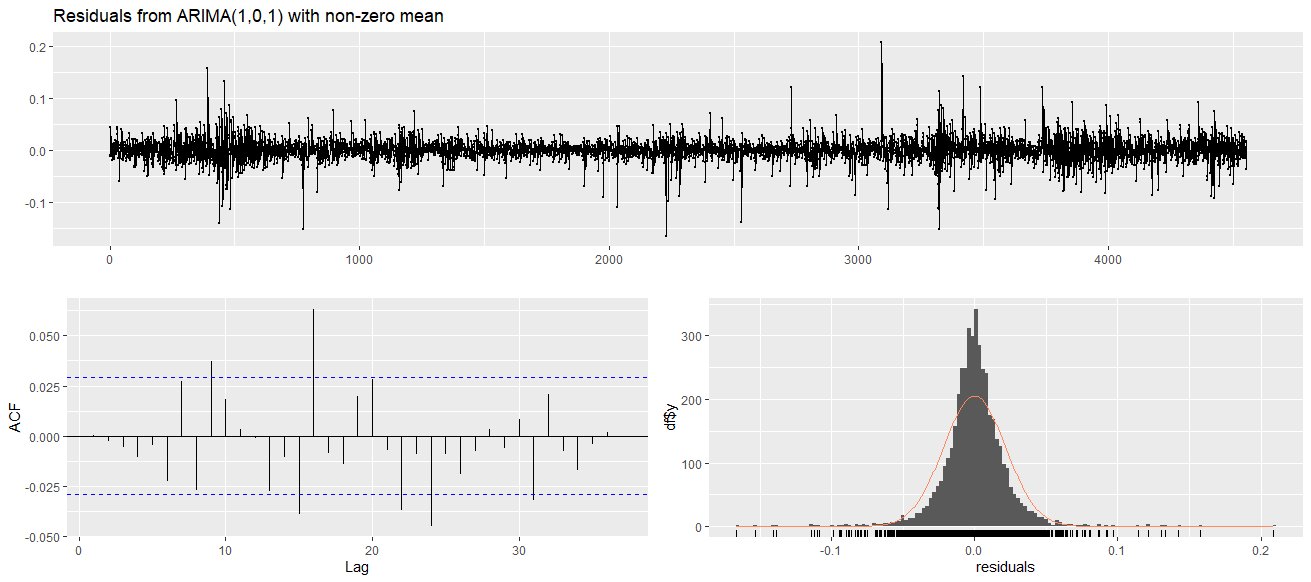
\includegraphics[width=0.7\linewidth]{content/plots/residual_plot_1_1.png}
		\caption{Residual Plots for the ARIMA(1,0,1) model for the Log Prices}
		\label{fig:residual_plot_1_1}
	\end{figure}
	
	\begin{figure}[!h]
		\centering
		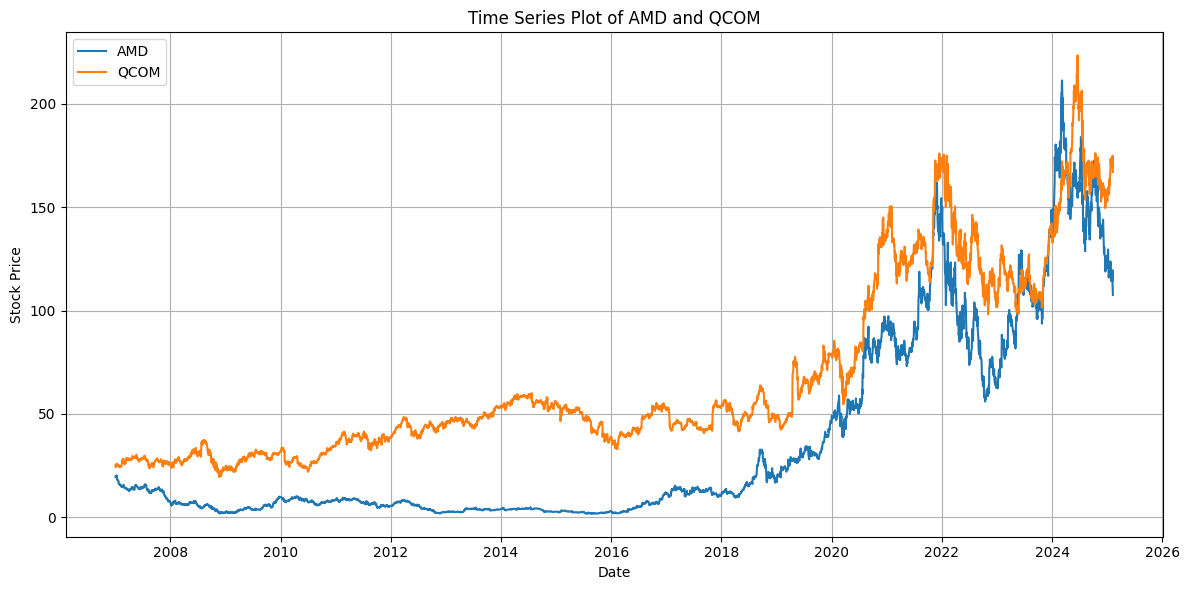
\includegraphics[width=0.8\linewidth]{content/plots/QCOM_AMD.png}
		\caption{Cumulative Returns of QCOM and AMD}
		\label{fig:amd_qcom_cumul_returns}
	\end{figure}
	
	\chapter{Tables}
	
	\begin{table}[ht]
		\centering
		\caption{Ljung-Box Test Model Fit}
		\begin{tabular}[t]{lccccc}
			\toprule
			   & Method &Lag order& t-statistic & $p$-value & Outcome  \\
			\midrule
			ARCH & Standard Residuals & 10 & 4.5922 & 0.9167 & No autocorrelation  \\				
			GARCH & Squared Residuals & 10& 9.6976 & 0.4674 & Stationary  \\				
			\bottomrule
		\end{tabular}\label{tab:ARCH_GARCH}
	\end{table}

\end{appendices}